\chapter{舱体设计}
\label{chp:cabin:begin}
\section{舱体设计}

\subsection{总体设计概况}

我们设计的基地是单体地基式饼状结构,整个基地是一个顶部凸起的矮平圆筒,和地面的接触方式为贴附,采用高强度的钛合金材料固定。除了太阳能电池板和大型机械(探险车等)之外所有功能单位均集中在此圆筒内。筒的顶部有采光机构,筒内分为上下两层:上层是植物舱,主要用于种植植物,下层是生活区,按功能不同划分为若干扇形区域。上层和下层之间有1米厚的隔离段,下层和地基之间有2米厚的隔离段,除去采光机构外的基地高度为13米,直径为28米。单层有效面积为615平方米,总体有效面积为1230平方米。

\subsection{设计细节说明}

1、采光机构:

采光机构处于舱体顶部,分为反射器、聚光器、固定器三部分。反射器具有类似于天文望远镜式的开合功能,它并非一块整体结构,而是分成 12 块独立可动的花瓣形状。闭合的反射器将完全遮挡植物区,起到隔绝尘埃和有害射线的作用。由于火星的昼夜变化和地球相近,而植物需要不间断的光照以维持基地的氧气浓度,花瓣状的反射器可以自动调节俯仰角度,确保植物区接收到的光强适合植物生长。所有的反射器由固定器与舱体外周连接,12个固定器等间隔地分布在舱体壁上,留出的间隔用于滤过风沙。由于火星表面的光强只有地球的 43\%,反射器能很好地增加光强。聚光器是位于采光机构顶部中间的光学仪器,用于将来自反射器的光线聚合并散射到植物区。

2、基地上层:

基地上层为植物舱主要用于种植植物,外环为1.4米宽的环形通道,内部被纵横相交宽0.8米的走廊分为4个扇形区域,这4个扇形区域的总面积为467平方米,用于种植植物。植物呈区块式种植,即4个区域又细分为各个种植某种植物的区域,具体种植的植物类型在植物的选育方面会专门提到。

基地上层的顶部是一个4米高的光滑透明凸面,分为内外两层,两层之间为真空状态。外层为高强度隔热透明玻璃,接触火星大气的那一面为光滑面,可以防止尘埃的滞留。内层为过滤面,具有防辐射的功能,可以过滤聚光器散射下来的太阳光线,滤除对植物有害的α射线、β射线等,保留对光合作用有益的波长部分。除此之外,内层玻璃的内面贴附有疏水性的光滑膜,防止植物呼吸产生的水汽在顶部凝结滞留,从而影响太阳光的透过。
舱体顶部细节见\cref{fig:cabin-root}。

\begin{figure}[H]
  \centering
  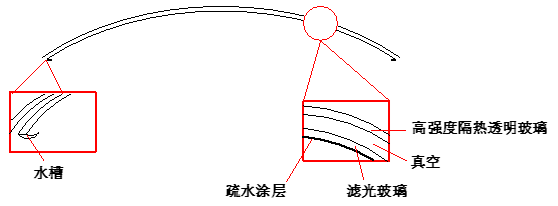
\includegraphics[width=0.8\textwidth]{figure/cabin-root.png}
  \caption{舱体顶盖细节图}
  \label{fig:cabin-root}
\end{figure}

为了收集植物呼吸作用产生的水汽,各种植区域内部还竖立了强导热金属采集板(见\cref{fig:collecting-broad}),采集板通过上下层之间的隔离带与外界低温联通,使其温度低于植物舱内部(约为5--10\si{\degreeCelsius}),采集板上附有和疏水性的滑膜,可以使植物舱内的水汽接触采集板后冷凝滑落到采集板下方的收集槽中,再进入管道进行处理和循环。

\begin{figure}[H]
  \centering
  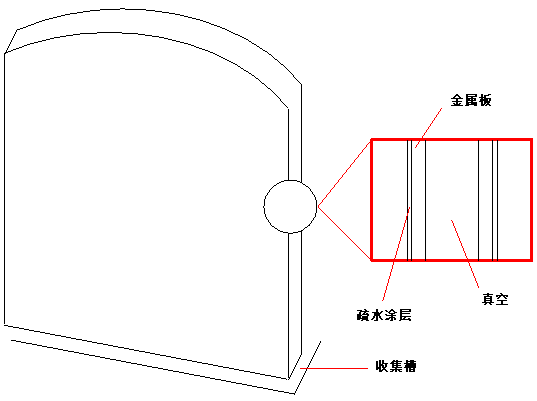
\includegraphics[width=0.6\textwidth]{figure/collecting-broad.png}
  \caption{采集板结构图}
  \label{fig:collecting-broad}
\end{figure}

3、基地下层:

基地下层是人类活动的主要区域,包含的功能区有:厨房/餐厅、起居室、实验室、中央控制室、娱乐室、浴室、仓库。为人们的生活和工作提供必要的场所。

4、隔离带:

基地有两个隔离带,分别处于基地上下层之间和基地下层与地基之间,厚度分别为1米和2米。隔离带主要功能有两个:一是将不同的舱室隔离,将基地下层与地基隔离;二是铺设了大量的管道、处理系统和循环系统,便于将收集的物质进行集中处理和循环供应,除此之外下层的隔离带还具备采集坑道内的地热能的功能。

为了便于人在基地上下层之间移动,我们在上下层配有若干通行设施。其中下层中央控制室中心配有一个升降梯,用于运输较重的货物到上层。除此之外,起居室、实验室、娱乐室、仓库均有一个爬梯可让人们在上下层之间通行。这些通行设施会穿过隔离带,但是与隔离带内部的结构是隔离开的,隔离带上会有密封滑盖门,在危急的时候会关闭以彻底隔离上下层。

5、基地外壳:

基地上层的外壳厚度为1米,下层外壳厚度为2米,这是从减少下层承重负荷的角度来考虑的。外壳的最外层为镀金的钛合金材料,减弱各种宇宙射线并起到支持的作用。中层为钛合金和高强度低导热纤维材料,主要起到隔热和密封的作用。内层为钛合金材料,主要起支持的作用。

6、关于舱体其他结构的一些参数:
\cref{tab:cabin-materials} 给出了舱体其他结构的一些参数,
舱体主要参数在 \crefrange{fig:zhengmian}{fig:xiaceng} 给出。
\begin{table}[H]
  \centering
  \caption{舱体材料}
  \label{tab:cabin-materials}
  \label{chp:cabin:end}
  \begin{tabular}{|>{\centering}m{0.2\textwidth}|m{0.3\textwidth}|m{0.4\textwidth}|}
    \hline
    部位 & 使用材料 & 参数 \tabularnewline
    \hline
    顶盖外层 & 高强度透明隔热玻璃 & 厚30厘米。\tabularnewline
    \hline
    顶盖内层 & 滤光玻璃 & 中心部分厚15厘米,逐渐往四周变厚,边缘厚度为25厘米。\tabularnewline
    \hline
    种植区 & 钛合金材料,表面覆有两层膜,内层为隔热的纤维膜,外层为疏水性的软膜
           & 支架侧面厚度为20厘米,底层为30厘米,预留种植深度为1米。(人的操作高度为1.3米)。
    纤维膜厚度为1厘米,软膜厚度为5毫米。\tabularnewline
    \hline
    采集板 & 金属层为高纯度的银,外层为疏水性软膜 & 金属层厚度为3厘米,软膜厚度为3毫米。\tabularnewline
    \hline
  \end{tabular}
\end{table}
